\chapter[Le stage \ensg]{Le stage}

\section{Généralités}

Dans la suite de ce rapport je vais me consacrer sur les deux missions principales que j’ai réalisées à Galigeo. La première est l’estimation d’un flux piéton à une adresse donné. (2.2) Ce n’est pas une mission réalisée pour un client en particulier, c’est une fonctionnalité qui a été ajouté dans la dernière version des logiciels SaS de Galigeo et est donc accessible pour tous les utilisateurs du service.

\paragraph*{}

La deuxième mission est une demande spécifique d’un client de Galigeo. J’ai eu accès à des données confidentiels à l’entreprise. Toutes les illustrations, schémas ou fragments de données, pour cette partie, seront donc fictifs

\paragraph*{}

Enfin, je terminerai rapidement sur deux autres missions clients, plus secondaires pour lesquels je rentrerai moins dans le détail.


\section{Prédiction de flux piéton}

\subsection{Mise en contexte}

Le flux piéton est une très bonne variable pour estimer le flux de consommateur potentiel qui passe chaque jour devant une enseigne commerciale. Il est donc essentiel pour une entreprise qui fournit des services de géomarketing, de pouvoir estimer au mieux cette variable.

\paragraph*{}

Jusqu’aujourd’hui, Galigeo s’appuyait sur des estimations calculées par une autre entreprise ce qui l’empêchait de corriger les biais et erreurs possibles. Elle n’avait pas la main sur les algorithmes d’estimations.

\paragraph*{}

Ma mission a donc été de réaliser cet algorithme d’estimation du flux moyen de piéton sur une année autour d’une adresse donnée et ce pour l'ensemble du territoire nationale.

\paragraph{}

Il a fallu néanmoins prendre en compte les contraintes techniques de l’entreprise, les biais qui pouvait être présent dans la donnée utilisée et l’efficacité de l’algorithme. Si les temps de calculs sont trop longs, l’expérience utilisateur risque d’être impactée mais il faut garder un modèle puissant afin de minimiser les erreurs de prédiction.

\subsection{La donnée}

Pour estimer ce flux piéton, nous allons nous appuyer sur des mesures quotidiennes que Galigeo achète à un fournisseur. En effet, Galigeo reçoit quotidiennement des positions de cellulaires sur l'ensemble du territoire métropolitain. Elle en reçoit environ XXXXXXX par mois, chacune correspond à un évènement de visite. Cette donnée est collectée via des applications mobiles qui sont autorisées à transmettre au fournisseur de Galigéo la position du smartphone. Les positions sont anonymes mais possède un identifiant de smartphone ce qui permet d'avoir aussi des informations de déplacements. La donnée brute est structurée comme ci-dessous:

\begin{table}[H]
    \centering
    \begin{tabular}{|l|l|}
    \hline
    \textbf{Attribut} & \textbf{Description}              \\ \hline
    idEvent           & Id de l'évènement                 \\ \hline
    uuid              & Id du smartphone                  \\ \hline
    latitude          & Latitude de l'évènement           \\ \hline
    longitude         & Longitude de l'évènement          \\ \hline
    accuracy          & Précision de la localisation      \\ \hline
    arrival           & Date d'arrivée à la localisation  \\ \hline
    departure         & Date de départ de la localisation \\ \hline
    \end{tabular}
    \caption{Résumé de la structure d'un évènement de visite}
\end{table}

\paragraph*{}

Nous avons également utilisé de la donnée économique pour enrichir notre modèle. En effet Open Street Map poropose une base open-source de POI structuré comme ci-dessous:

\begin{table}[H]
    \centering
    \begin{tabular}{|l|l|}
    \hline
    \textbf{Attribut} & \textbf{Description}                                  \\ \hline
    id\_poi           & Id du poi                                             \\ \hline
    type              & Nature du POI (Magasins, Restaurants, Epiceries, ...) \\ \hline
    latitude          & Latitude du POI                                       \\ \hline
    longitude         & Longitude du POI                                      \\ \hline
    \end{tabular}
    \caption{Structure d'un POI}
\end{table}

\paragraph*{}

Il était également intéressant de rajouter de la donnée démographique à notre modèle pour cela nous avons utilisé les données de population de l'INSEE agrégé au niveau des IRIS géographiques.

\paragraph*{}

Nous allons utiliser des algorithmes de Machine Learning pour estimer ce traffic piéton donc il nous faut des données vraies mesuré sur le terrains afin d'entraîner un modèle. Galigeo possède plus de 11000 mesures répartient de façon homogène sur le territoire même si la plus part d'entre elles sont en milieu urbain.

\begin{figure}[H]
    \centering
    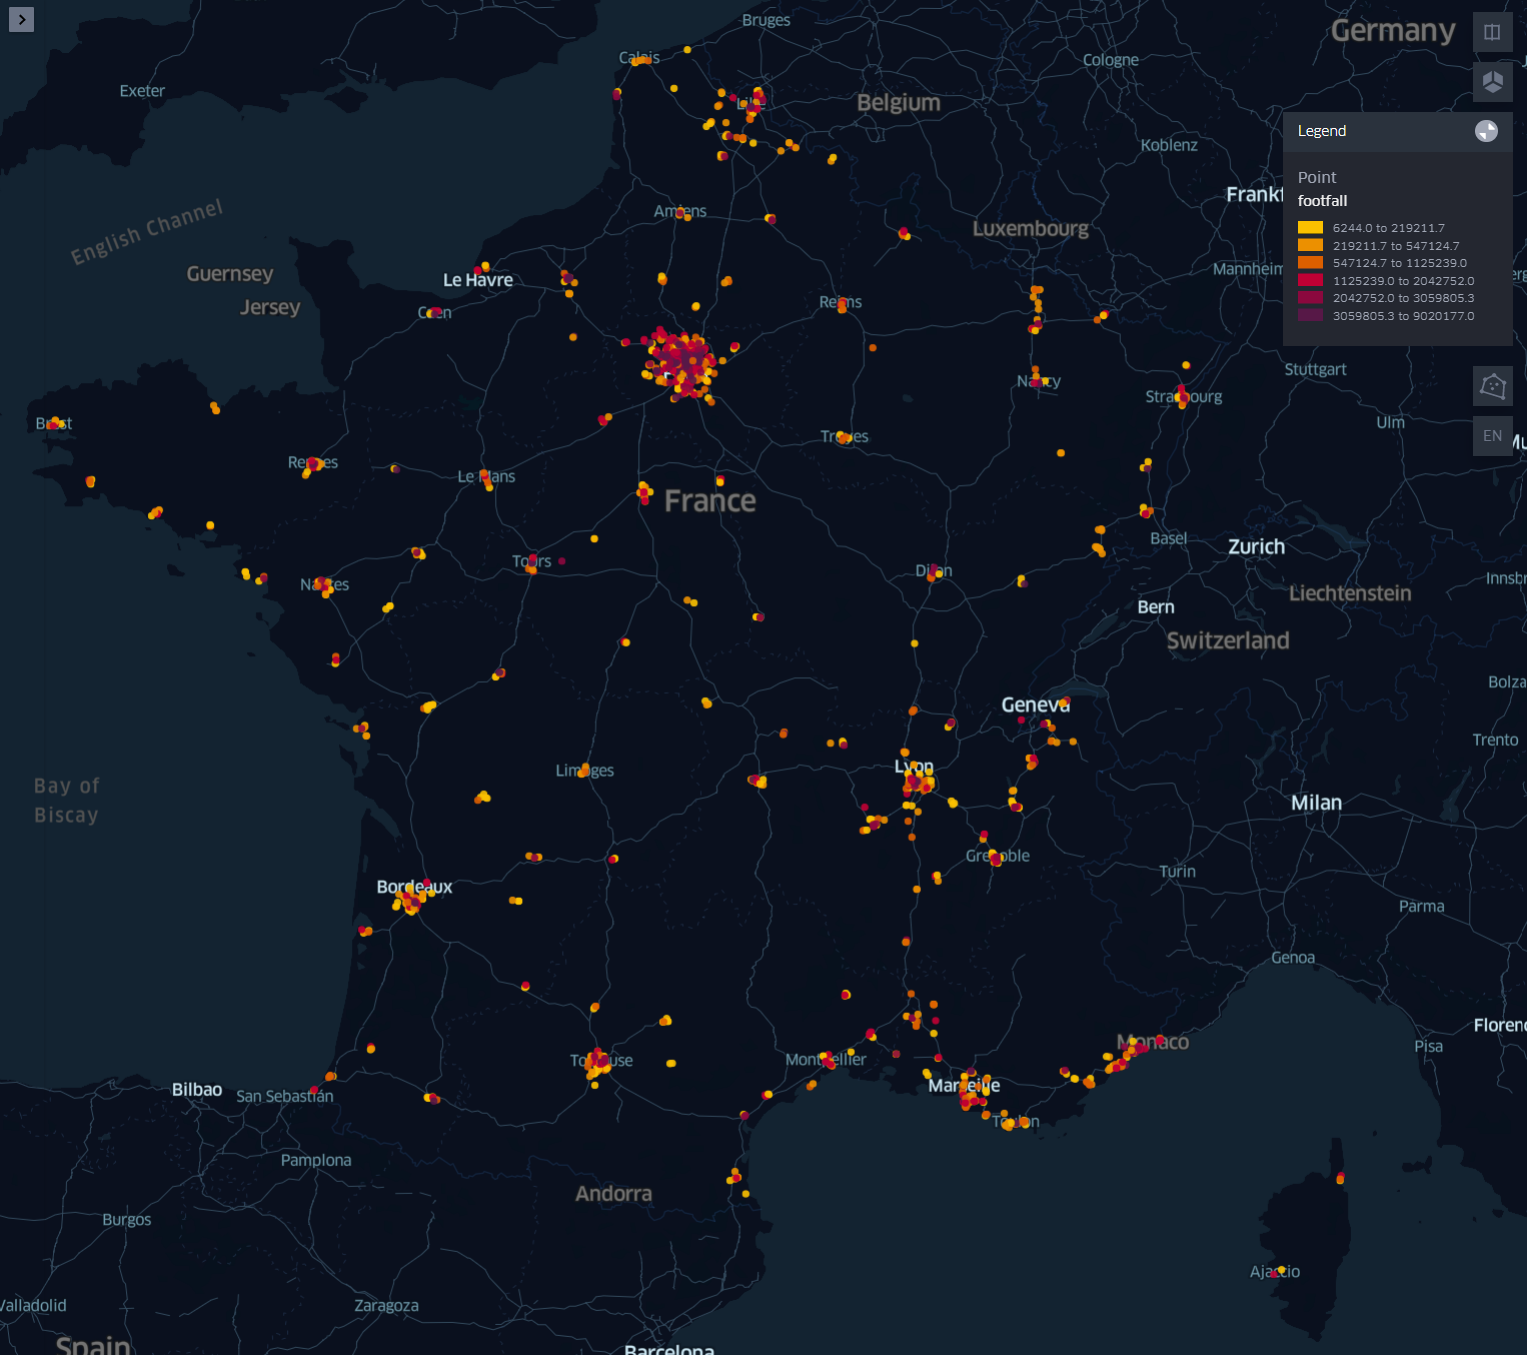
\includegraphics[width=\linewidth]{images/graphs/map_of_label_footfall.png}
    \caption{Carte des données d'entraînement}
    \label{fig:footfallmap}
\end{figure}

\subsection{Technologies utilisées}

\subsubsection{Agrégation spatiale}

Une fois que nous avons l'ensemble de nos donnée on remarque qu'elles se distingue en deux groupe de part leur nature. Les données ponctuelles (\'Evènements de visites, POI, etc.) et les données surfaciques (Population par IRIS). Pour homogéniser notre donnée et simplifier les futurs calcul il est important de segmenté l'espaces et ajouter un index spatial à nos données.

Nous nous sommes dirigé vers la solution des hexagones H3 \cite{Uber_H3} développé par Uber. C'est un système d'indexation géospatiale qui constitue un pavage hexagonale de la sphère multi-echelles et dont les index sont hierarchiques.

Dans notre cas c'est la solution optimale car nous pouvons l'utiliser pour joindre nos données disparates, le format hexagonale facilite la modélisation des flux et est bien adapté pour appliqué le machine learning aux données géospatiales. 

% Image of the offices
\begin{figure}[H]
    \centering
    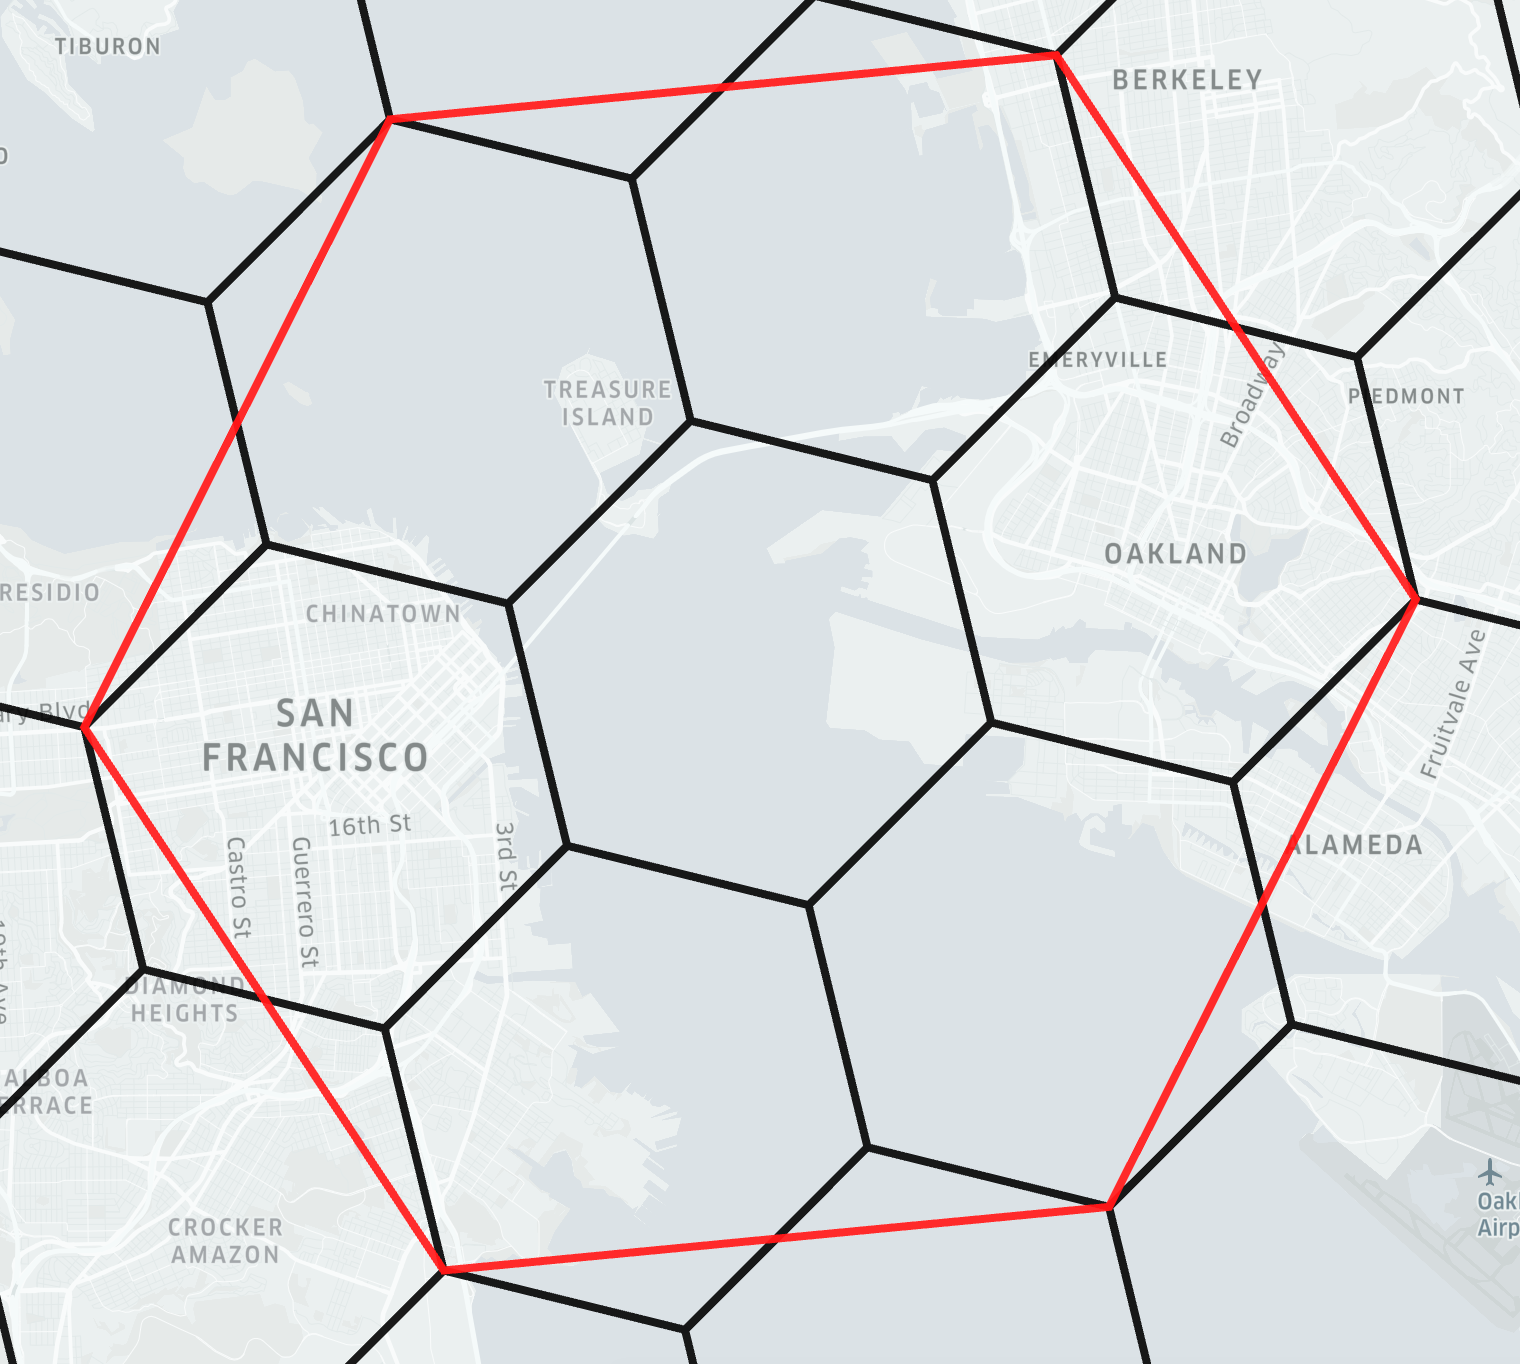
\includegraphics[width=7cm]{images/graphs/h3-multiscale.png}
    \caption{Principe de multi-echelles des cellules H3}
    \label{fig:celluleh3}
\end{figure}

\begin{figure}[H]
    \centering
    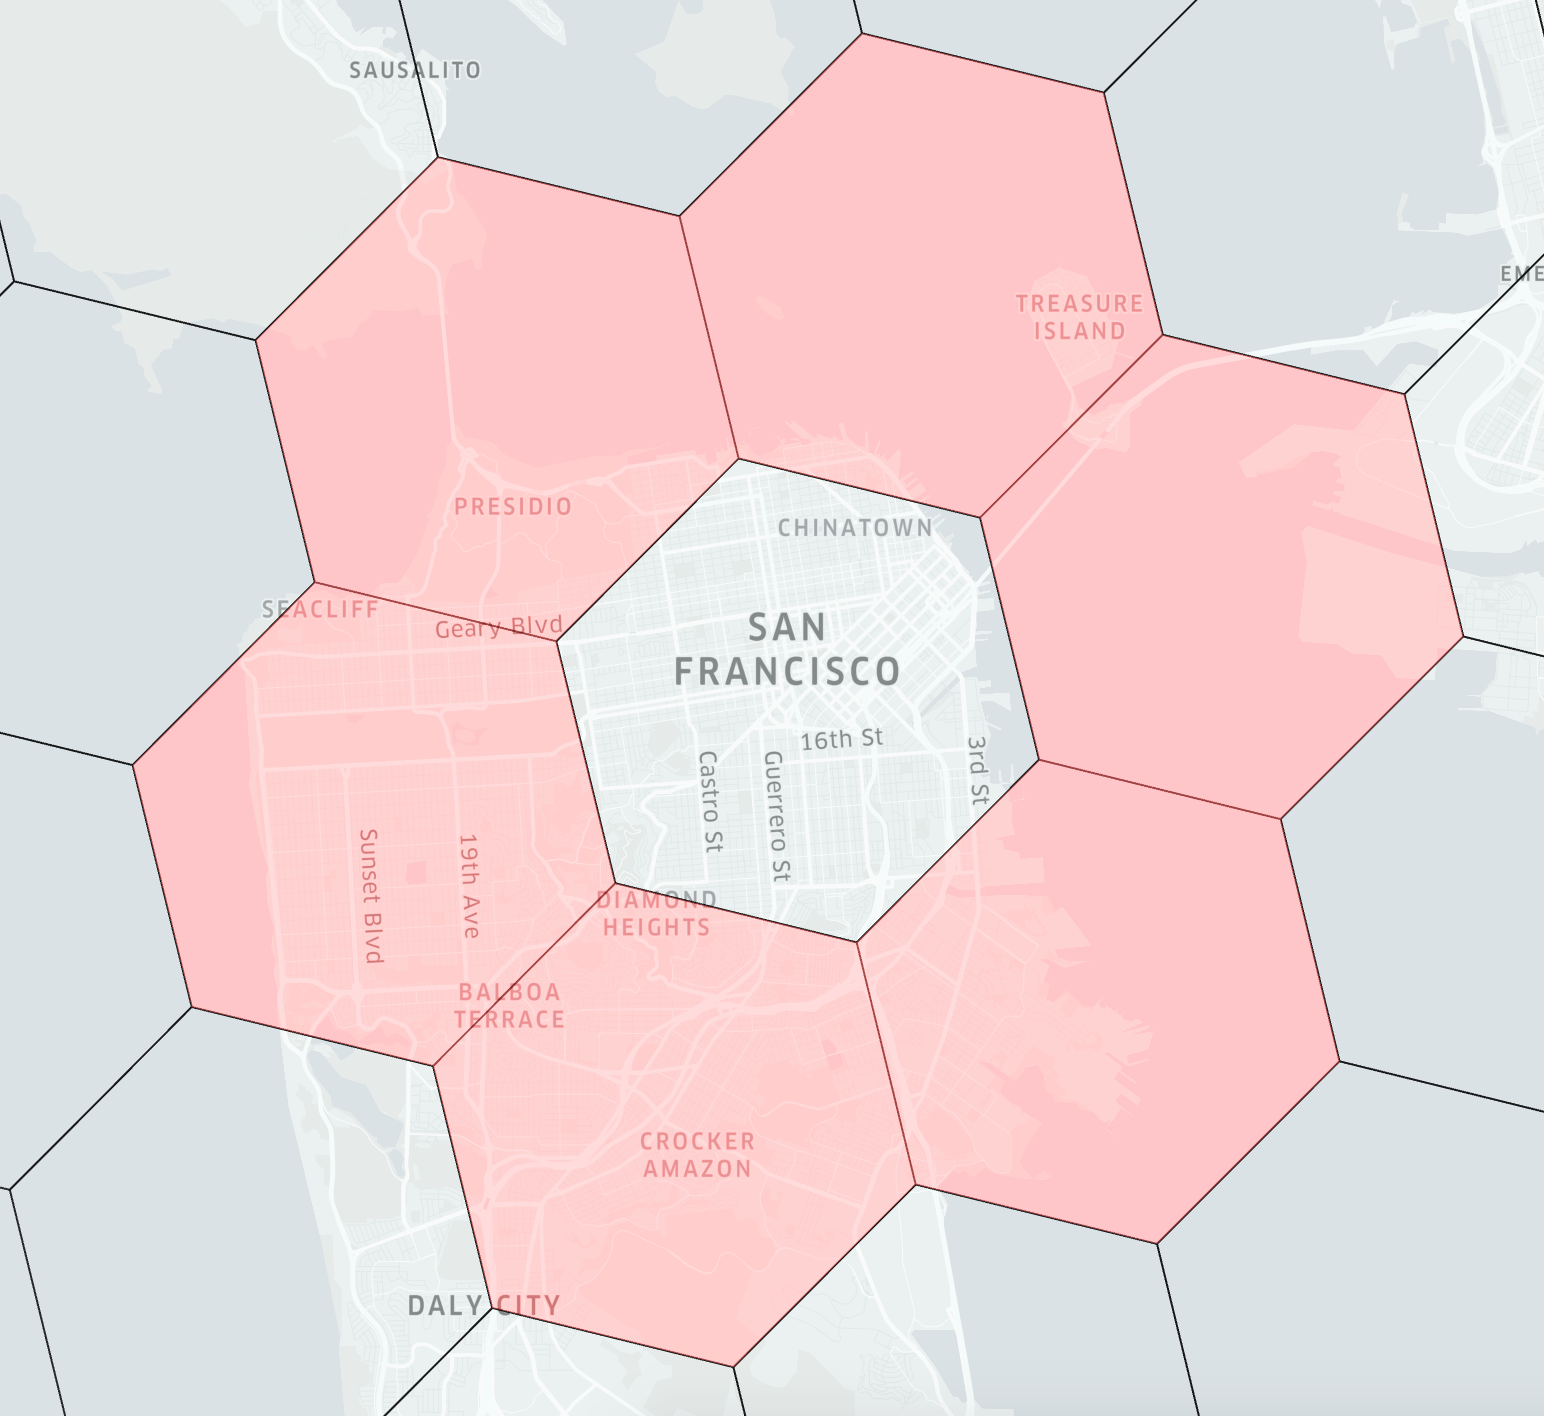
\includegraphics[width=7cm]{images/graphs/h3-ring.png}
    \captionsetup{justification=centering}
    \caption{Les 6 voisins d'une cellule H3 se rapproche d'un cercle, utile pour la modélisation de flux}
    \label{fig:celluleh3ring}
\end{figure}

Pour notre part on choisira le niveau d'échelle 12, ce qui correspond environ à un hexagone de X mètres de rayon.

\subsubsection{Infrasture de base de donnée}

A compléter

\subsection{Entraînement et Tuning du modèle}

\subsection{Résultats}

\subsection{\'Evolutions possibles}

\section{Prédiction de chiffre d'affaire}

\subsection{Contexte}

\subsection{Données disponibles}

\subsection{Structure du modèle}

\subsection{Résultats}

\section{Autres missions}

\subsection{Analyse de données - Base de donnée nationale des Bâtiments}

\subsection{Data engineering - Scrapping et automatisation de chaîne d'acquisition de données}